% use paper, or submit
% use 11 pt (preferred), 12 pt, or 10 pt only

\documentclass[letterpaper, preprint, paper,11pt]{AAS}	% for preprint proceedings
%\documentclass[letterpaper, paper,11pt]{AAS}		% for final proceedings (20-page limit)
%\documentclass[letterpaper, paper,12pt]{AAS}		% for final proceedings (20-page limit)
%\documentclass[letterpaper, paper,10pt]{AAS}		% for final proceedings (20-page limit)
%\documentclass[letterpaper, submit]{AAS}			% to submit to JAS

\usepackage{bm}
\usepackage{amsmath}
\usepackage{subfigure}
%\usepackage[notref,notcite]{showkeys}  % use this to temporarily show labels
\usepackage[colorlinks=true, pdfstartview=FitV, linkcolor=black, citecolor= black, urlcolor= black]{hyperref}
\usepackage{overcite}
\usepackage{footnpag}			      	% make footnote symbols restart on each page
\usepackage{float}
\usepackage{color}



\PaperNumber{XX-XXX}

% TO ADD:
% BREAK-UP CRITERIA
% NON-FRAG CASE
% pure sine v actual


\begin{document}

\title{\textsf{\textbf{Induced Fragmentation of Asteroids during Close Encounters}}}
\author{\textsf{Bryan Tester}\thanks{PhD student at University of Strathclyde, \textbf{\emph{Give more details here}} United Kingdom}
\ and \textsf{Prof. Massimiliano Vasile}\thanks{Professor at University of Strathclyde,\textbf{\emph{Give more details here}} United Kingdom}}

\maketitle{} 		


\begin{abstract}
\textbf{\emph{I think the abstract is too short. It needs to be at least 100 words and needs to be the same as what you submitted as first paragraph of the extended abstract}}. We consider the behaviour of rotating binary asteroids as they pass through Earth's Hill sphere, with primary interest in the effect the tidal force has on the interaction between the two components of the binary and their post-encounter trajectories. We focus on contact binary asteroids bound by a regolith bridge, using both direct numerical simulation and an analytical approach. \textbf{\emph{A little bit more detail on what you are doing and what kind of results you are presenting}}.
\end{abstract}

\section{Introduction}
Radar observations suggest that a significant portion of Asteroids with Earth-crossing orbits are binary systems, consisting of two components in contact with or in close proximity to each other. As shown by work such as that of Farinella \textit{et al} \cite{binaryevo} in the early 1990s, gravitational encounters can significantly alter the orbits and integrity of binary asteroids. Clearly, it is important to be able to accurately predict the motion of these bodies to give best probabilities of any possible Earth collision event. The work presented here is inspired by that of Borum \textit{et al}\cite{exchange}. In our work, we revisit some of the previously discussed cases and then expand to include “Contact Binaries” (single asteroids formed primarily by two large boulders); we consider both gravitationally bound pairs and those bound by a regolith bridge, as illustrated in Figure ~\ref{fig:Pic} (this mechanism is similar to that discussed by Sanchez \& Scheeres \cite{dustbound}). \textbf{\emph{Perhaps one more sentence about what a regolith bridge is and what do the colors mean in the figure}}. We also model an attempted deflection of the asteroid prior to the close encounter. \textbf{\emph{Our analysis uses both an analytical approach and numerical simulations.}}. Our analysis has been performed using both numerical simulations and by taking an analytical approach.
\textbf{\emph{Expand a little bit more}}.

\begin{figure}[H]
\centering
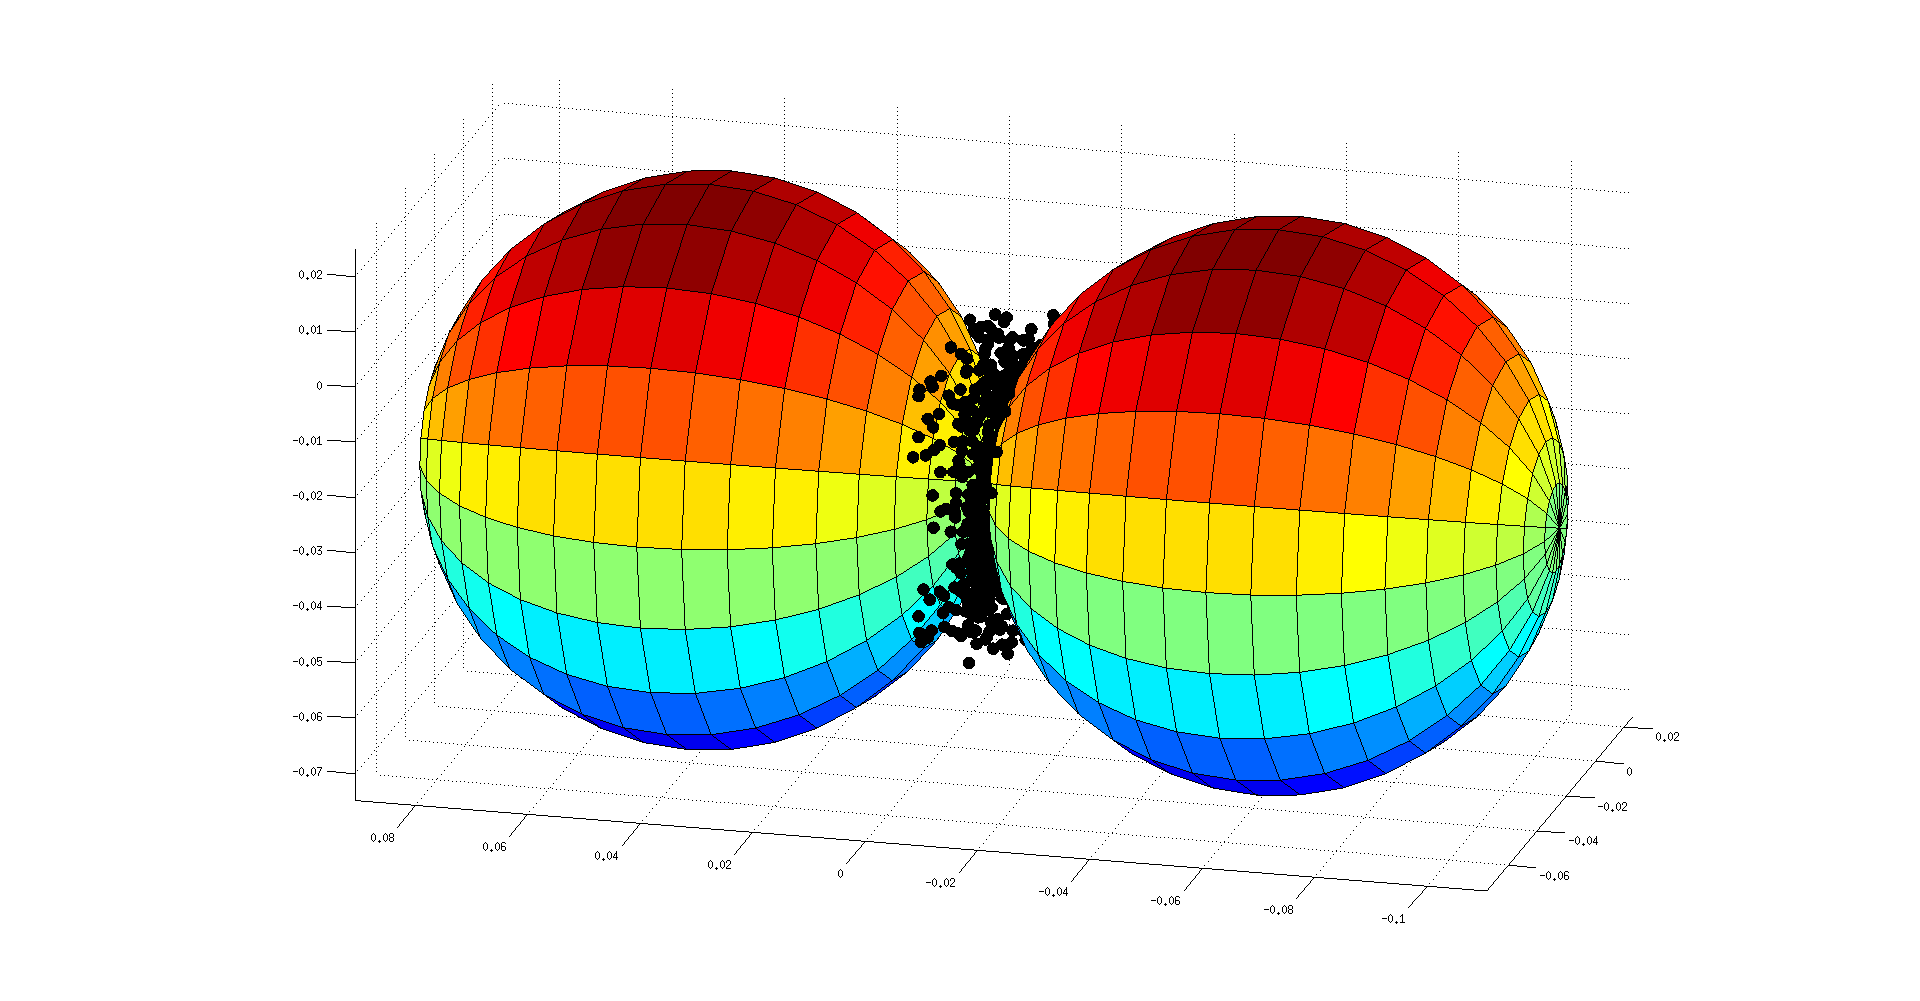
\includegraphics[width=0.6\textwidth]{binary_3d.eps} 
\caption{Simulation of two 10 cm diameter spheres joined by a finer regolith bridge.} 
\label{fig:Pic}
\end{figure} 

\section{Analytical Approach}
\subsection{Equations of Motion}

The analytical approach to characterising the system is based upon the full equations of motion in a rotating reference frame, with the angular velocity of the reference frame, $\vec{\omega}$, varying such that the barycentre of the system remains at a constant angle to the Earth. The resulting equations can be split into two separate parts that detail the motion of the barycentre and the relative motion of the binary components, respectively. $\vec{R}$ denotes the position of barycentre of the system with respect to Earth; the binary components considered are identical, both with mass $m$ and positions given by $\vec{R}\pm\vec{\rho}$. \textbf{\emph{Reframe the previous sentence}}. By the definition of the reference frame, $\vec{R}$ has constant direction and varies only in magnitude. We start by working with the equation of motion for $\vec{R}$:

\begin{equation}
\ddot{\vec{R}} = \frac{-GM_\oplus}{\|\vec{R}\|^{3}}\vec{R}+\vec{\omega}\times(2\dot{\vec{R}}+\vec{\omega}\times\vec{R})+\dot{\vec{\omega}}\times\vec{R}
\end{equation}

As stated earlier, the definition of $\vec{\omega}$ in our reference frame implies that the direction of $\vec{R}$ is constant. Thus, any components of $\vec{\ddot{R}}$ orthogonal to $\vec{R}$ must be zero. This implies the following definiton of the magnitude of $\vec{\ddot{R}}$, along with Eq. (3) \textbf{\emph{Put equation reference here}}. (which is equivalent to the conservation of angular momentum): 
\begin{equation}
\ddot{R} = \frac{-GM_\oplus}{R^{2}}+\omega^{2}R
\end{equation}
\begin{equation}
2\vec{\omega}\times\dot{\vec{R}}+\dot{\vec{\omega}}\times\vec{R}=0
\end{equation}
Since we consider no forces acting outside of the orbital plane, the direction of $\vec{\omega}$ must remain constant. We consider the conservation of angular momentum to obtain an equation for $\omega$: \textbf{\emph{Should not this be an $\vec{\omega}$}. Also, should the equation not have a number?}.
\begin{equation}
\notag\frac{\partial\left(R^{2}\omega\right)}{\partial t} = 2R\dot{R}\omega + R^{2}\dot{\omega} = 0 \implies R^{2}\omega = constant
\end{equation}
Assuming initial values for $R_0$ and $\omega_0$ at some time $t_0$, we get the following:
\begin{equation}
\omega = \frac{R_0^{2}\omega_0}{R^{2}}
\end{equation}

Now, we can move on to consider the equation of motion for the position of the binary components relative to the centre of mass, $\vec{\rho}$: 
\begin{equation}
\ddot{\vec{\rho}} = \left[\frac{-Gm}{4\|\vec{\rho}\|^{3}}+F(\vec{\rho})\right]\vec{\rho}+\vec{\omega}\times(2\dot{\vec{\rho}}+\vec{\omega}\times\vec{\rho})+\dot{\vec{\omega}}\times\vec{\rho}+{GM_\oplus}\left[\frac{\vec{R}}{\|\vec{R}\|^{3}}-\frac{\vec{R}+\vec{\rho}}{\|\vec{R}+\vec{\rho}\|^{3}}\right]
\end{equation}
We make the assumption that the pair remains in a mutual circular orbit until a fragmentation event. As such, by considering only components in the $\vec{\rho}$ direction, we obtain an equation describing the forces acting along $\ddot{\rho}$ and hence responsible for the binding of the pair ($\theta$ being the angle between $\vec{R}$ \& $\vec{\rho}$ at a given time). \textbf{\emph{Take care of and maintain the notations in the text}}.
\begin{equation}\label{eq:rdd}
\ddot{\rho} = \left[\frac{-Gm}{4\rho^{2}}+F(\rho)\right]+2\omega\dot{\rho}+\omega^{2}\rho+{GM_\oplus}\left[\frac{\cos\theta}{R^{2}}-\frac{R\cos\theta+\rho}{(R^{2}+2R\rho\cos\theta+\rho^{2})^\frac{3}{2}}\right]
\end{equation}

 




\section{Numerical Simulations}
The numerical simulations are run using a custom multi-body code that includes full inter-particle gravitational interactions, London dispersion forces and Soft-Body collisions similar to those implemented in \textit{PKDGRAV} by Schwartz \textit{et al}\cite{soft}.
Previous work considering the orbits of binary and rubble pile asteroid has only considered gravitational interactions between the components. 
Initially, we ran simulations comprised only of the two binary components and Earth. Encounters with a range of Earth-Asteroid two-body energies and varying binary asteroid rotation speed were simulated. The binary components are initially placed in a mutual circular orbit in each case with the force between them artificially varied to simulate the effects of a regolith bridge binding the two components.
\begin{figure}[H]
\centering
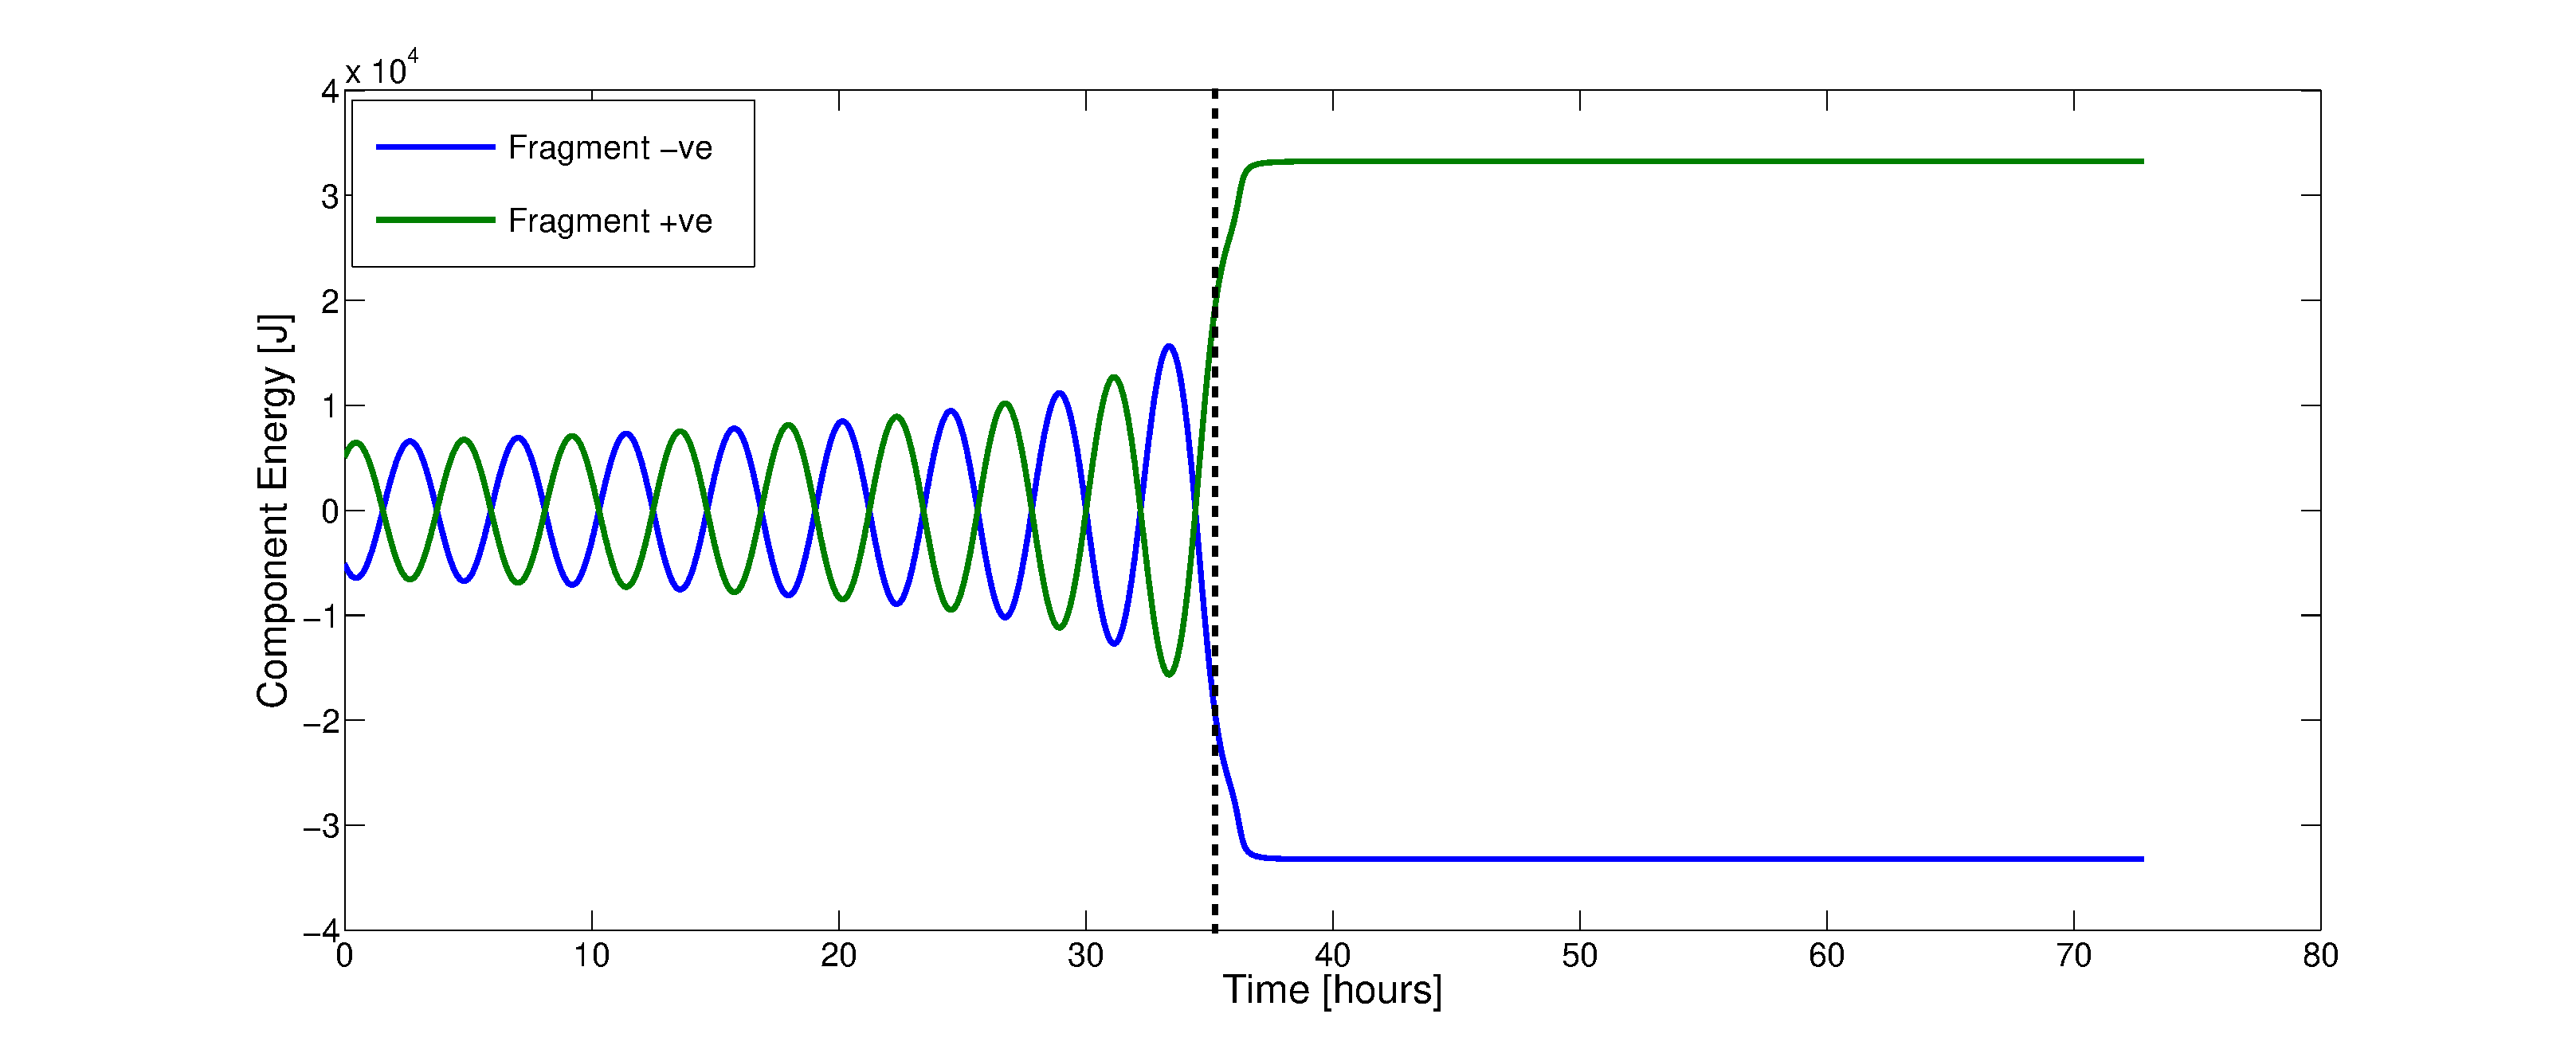
\includegraphics[width=\textwidth]{binary_num.eps} 
\caption{Plots of the Gravitational potential and kinetic energy of both components of the binary from numerical simulations.} 
\label{fig:Num}
\end{figure}
 Figure ~\ref{fig:Num} shows the output of such a simulation for a binary on a Parabolic trajectory; after the fragmentation one components is "captured" (having its orbital energy reduced below zero) and the other escapes (gaining orbital energy).  
 
\subsection{Analytical comparisons}

Using the set of equations derived earlier, we can make some estimations on the behaviour of the binary asteroid; namely whether or not a fragmentation event is expected and if so at what time it is expected to occur.

If we consider the fragmentation event to be instantaneous and that the radius of the binary orbit remains constant up until this point, we can neglect the term involving $\dot{\rho}$ in equation~\ref{eq:rdd}. The resulting equation has two important parts; namely the attractive and repulsive terms.
\begin{equation} \label{eq:attr}
\ddot{\rho}_{attr} = \left[\frac{-Gm}{4\rho^{2}}+F(\rho)\right]
\end{equation}
\begin{equation} \label{eq:rep}
\ddot{\rho}_{rep} = \omega^{2}\rho+{GM_\oplus}\left[\frac{\cos\theta}{R^{2}}-\frac{R\cos\theta+\rho}{(R^{2}+2R\rho\cos\theta+\rho^{2})^\frac{3}{2}}\right]
\end{equation}

Since we are only using these equations as a comparison to the computational simulations, rather than using an analytical solution for $R$ we evaluate $\omega$ in each frame of the simulation using the corresponding numerical value of $R$. Assuming the rotation rate is balanced with the attractive force between the binary components such that the orbit is circular when in free space, any effective repulsive force between the two components introduced by the influence of a third body would alter the orbit into an elliptical one or if strong enough eliminate the possibility of any stable orbit. If the strength of the repulsive force is greater than that of the attractive, the net effective force between the pair is repulsive and as such fragmentation is inevitable. 

Figure ~\ref{fig:Analy} shows a plot of the ratio between the Repulsive and Attractive force components, given in equations~\ref{eq:rep} and~\ref{eq:attr} respectively. Also plotted is the ratio between current and final total energy of one of the binary components (values from the same numerical simulation). \textbf{\emph{How do we know the final energy at current time?}}. The break-up is observed as the energy trace transitions from the oscillating regime to a steady state.
\begin{figure}[H]
\centering
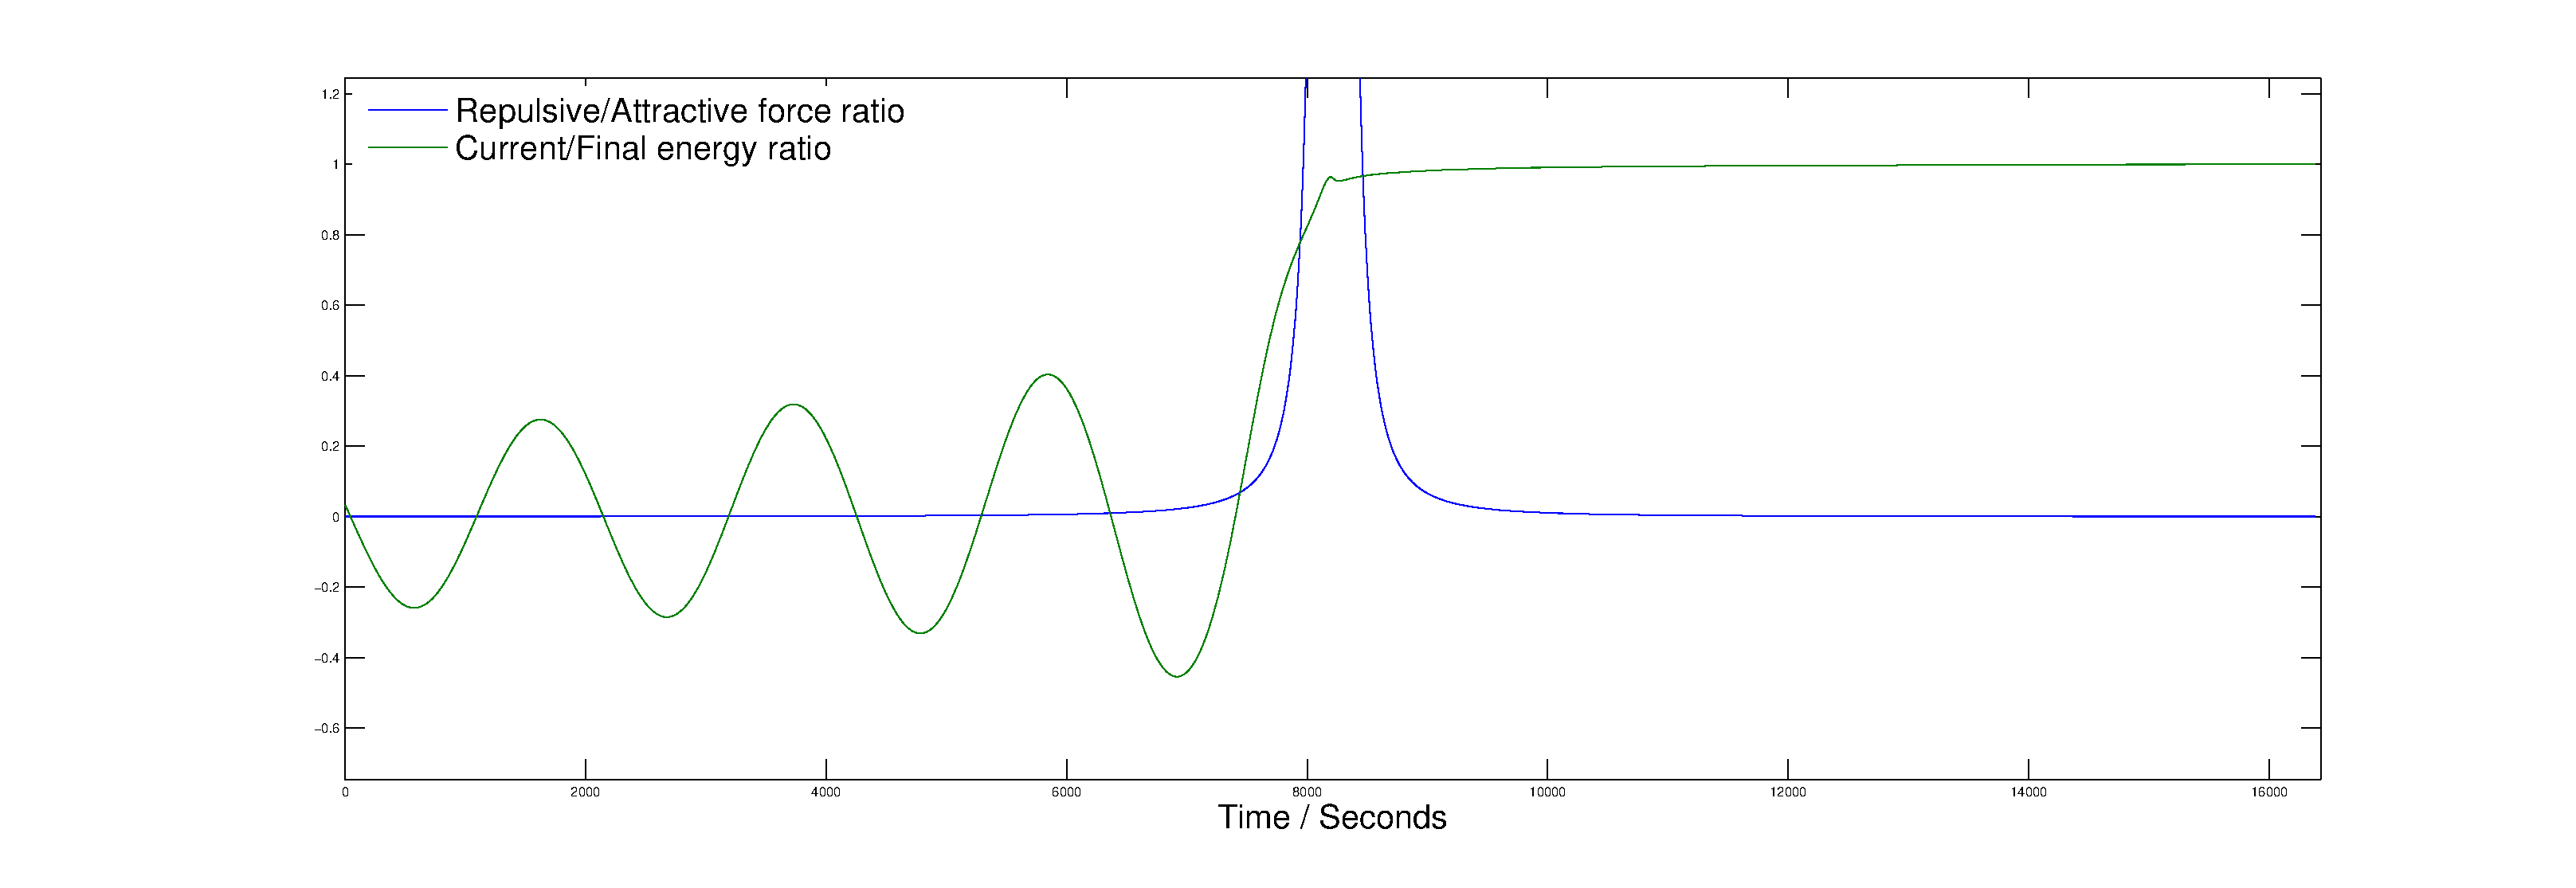
\includegraphics[width=\textwidth]{binary_analy.eps} 
\caption{Plots of the ratio between attractive and repulsive forces predicted by analytical model and Gravitational potential and kinetic energy of 1 component of the binary as a fraction of its final energy state from numerical simulations.} 
\label{fig:Analy}
\end{figure} 


Also, as can be seen in equation~\ref{eq:rep}, the repulsive effective force between the components has a dependence on the angle $\theta$. Figure ~\ref{fig:phase} shows the total energy plots for one component in a binary system over the course of an encounter with the Earth, with the value of $\theta$ at the start of the simulation varied; as can be seen there is a significant variation in the final energy. 
 \begin{figure}[H]
\centering
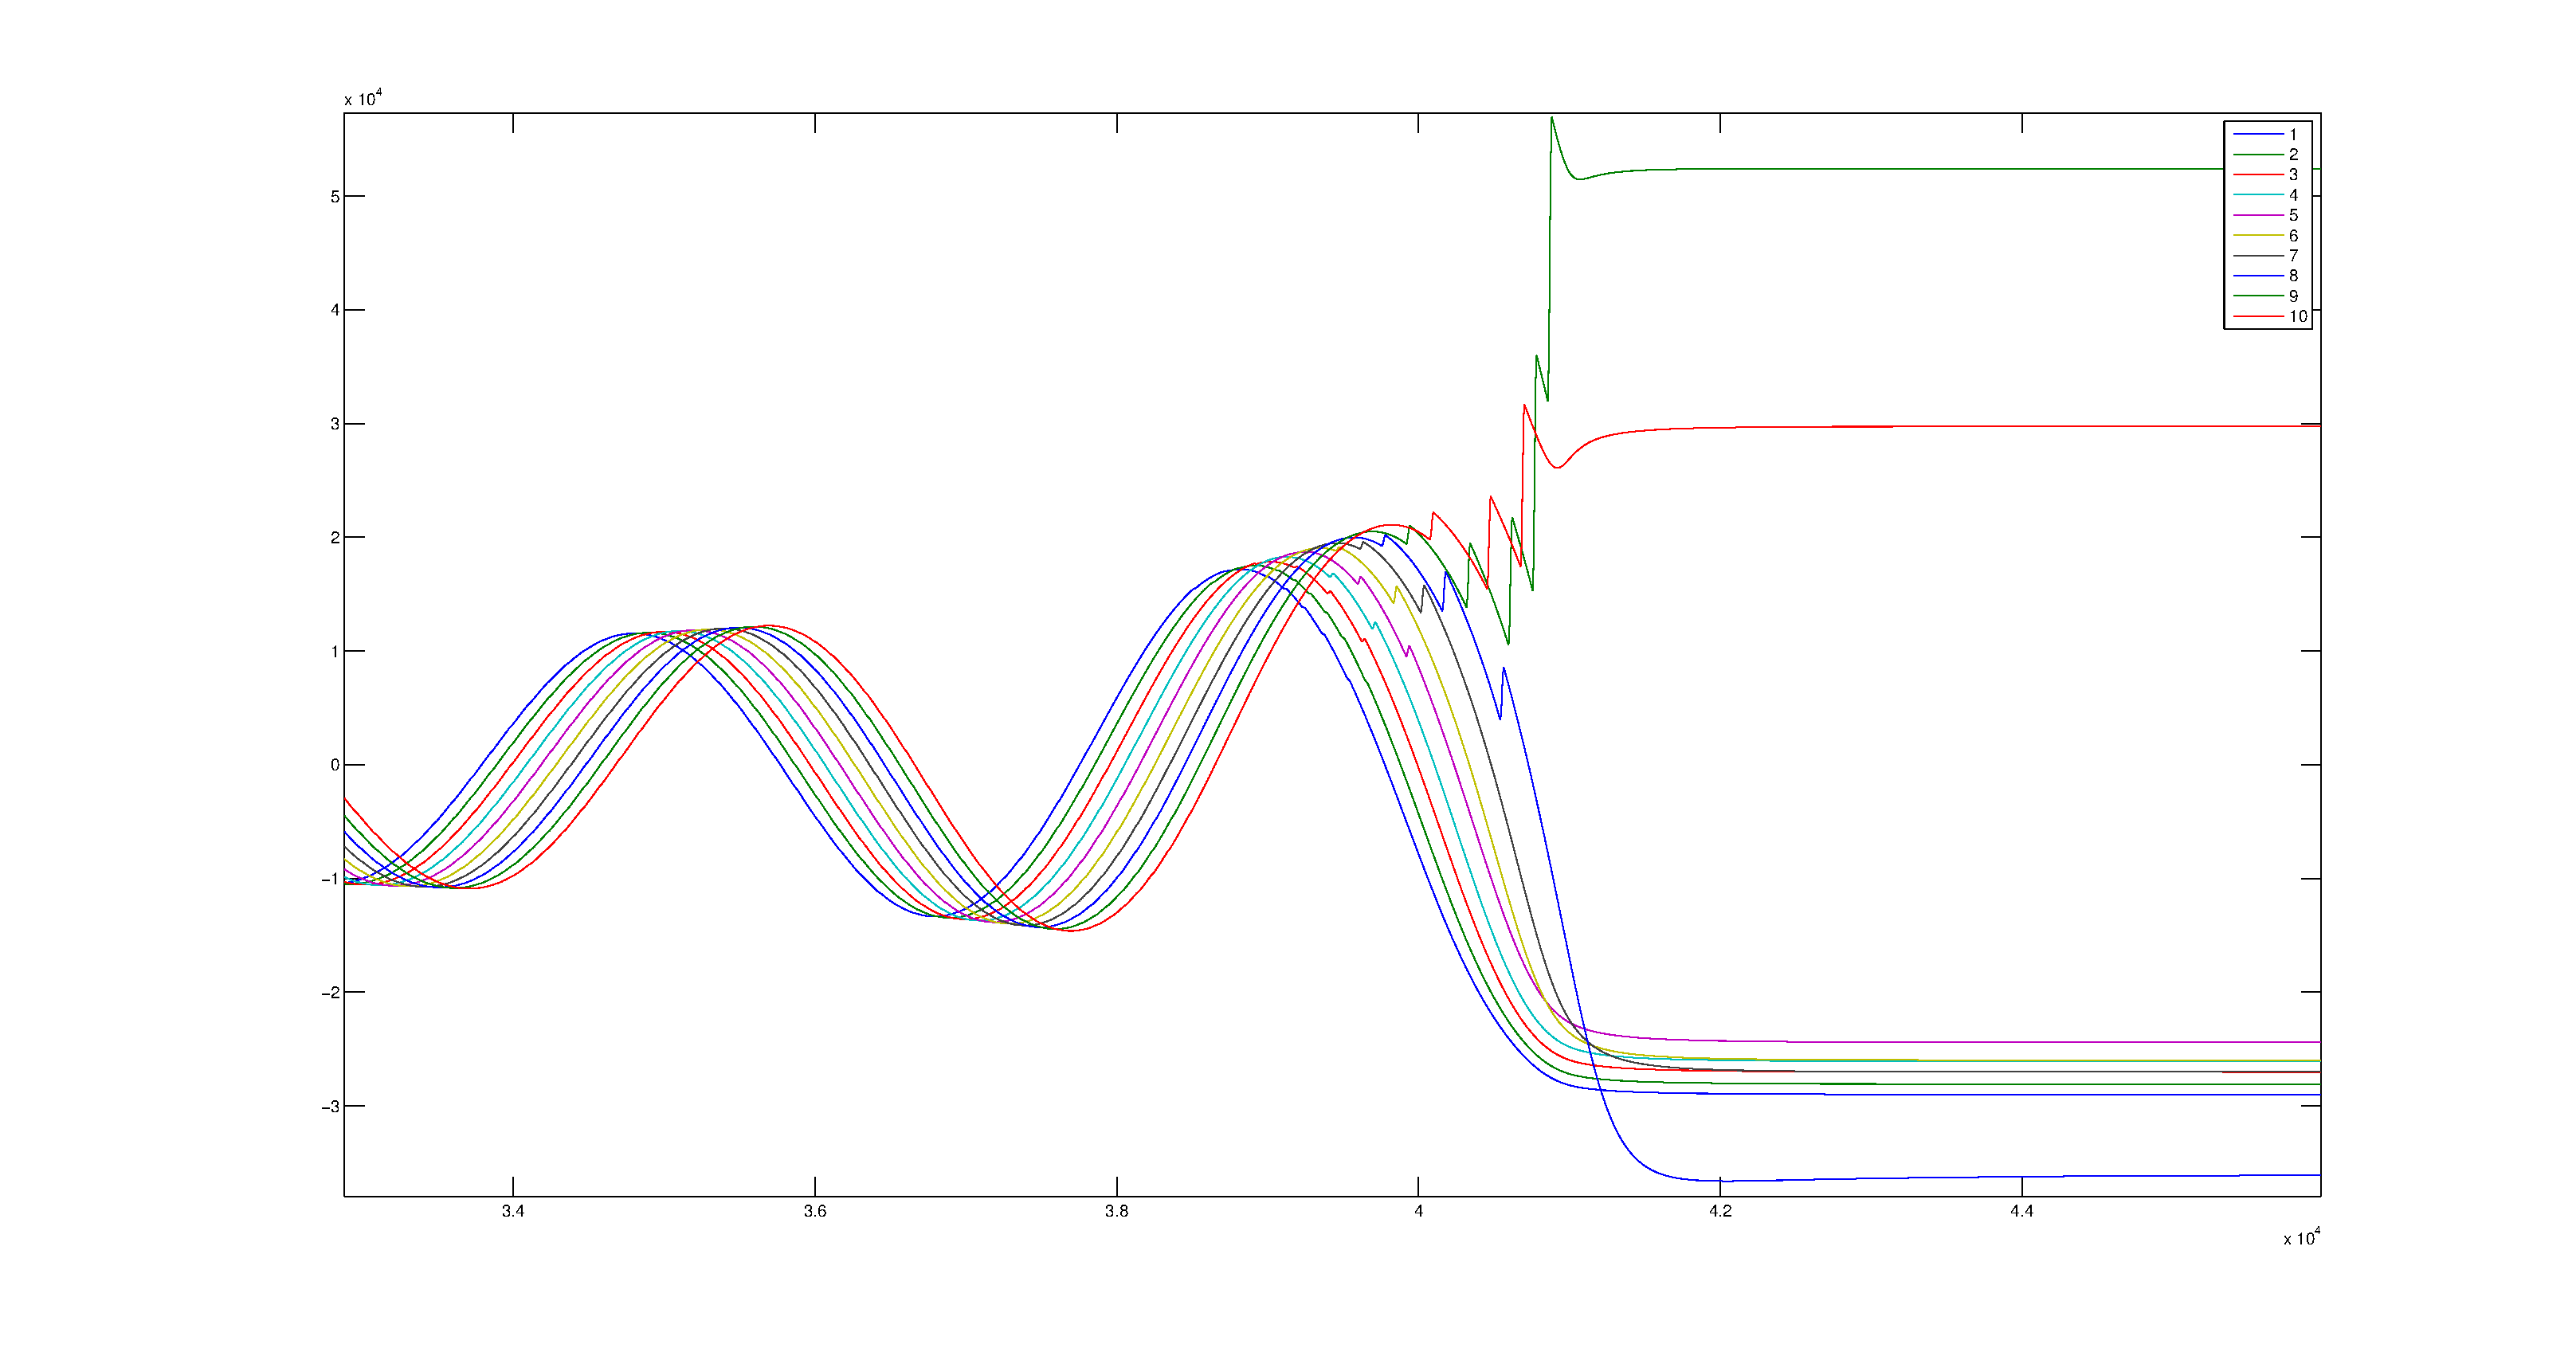
\includegraphics[width=\textwidth]{phasing_2.eps} 
\caption{Plots of the total energy for varying starting angle $\theta$.} 
\label{fig:phase}
\end{figure} 

The equations used here have been derived under the assumption that the rotation rate and radius of the binary pair remains constant until the fragmentation event occurs. To give an indication of the level of accuracy of this assumption, figure~\ref{fig:sin} shows the total energy of one of the binary components plotted alongside a sine wave of the same period as the binary orbit. It can be seen that the orbital period begins to increase as the binary gets closer to the earth; however for the cases considered the slow-down is only $1\%$ of the orbital period. 
\begin{figure}[H]
\centering
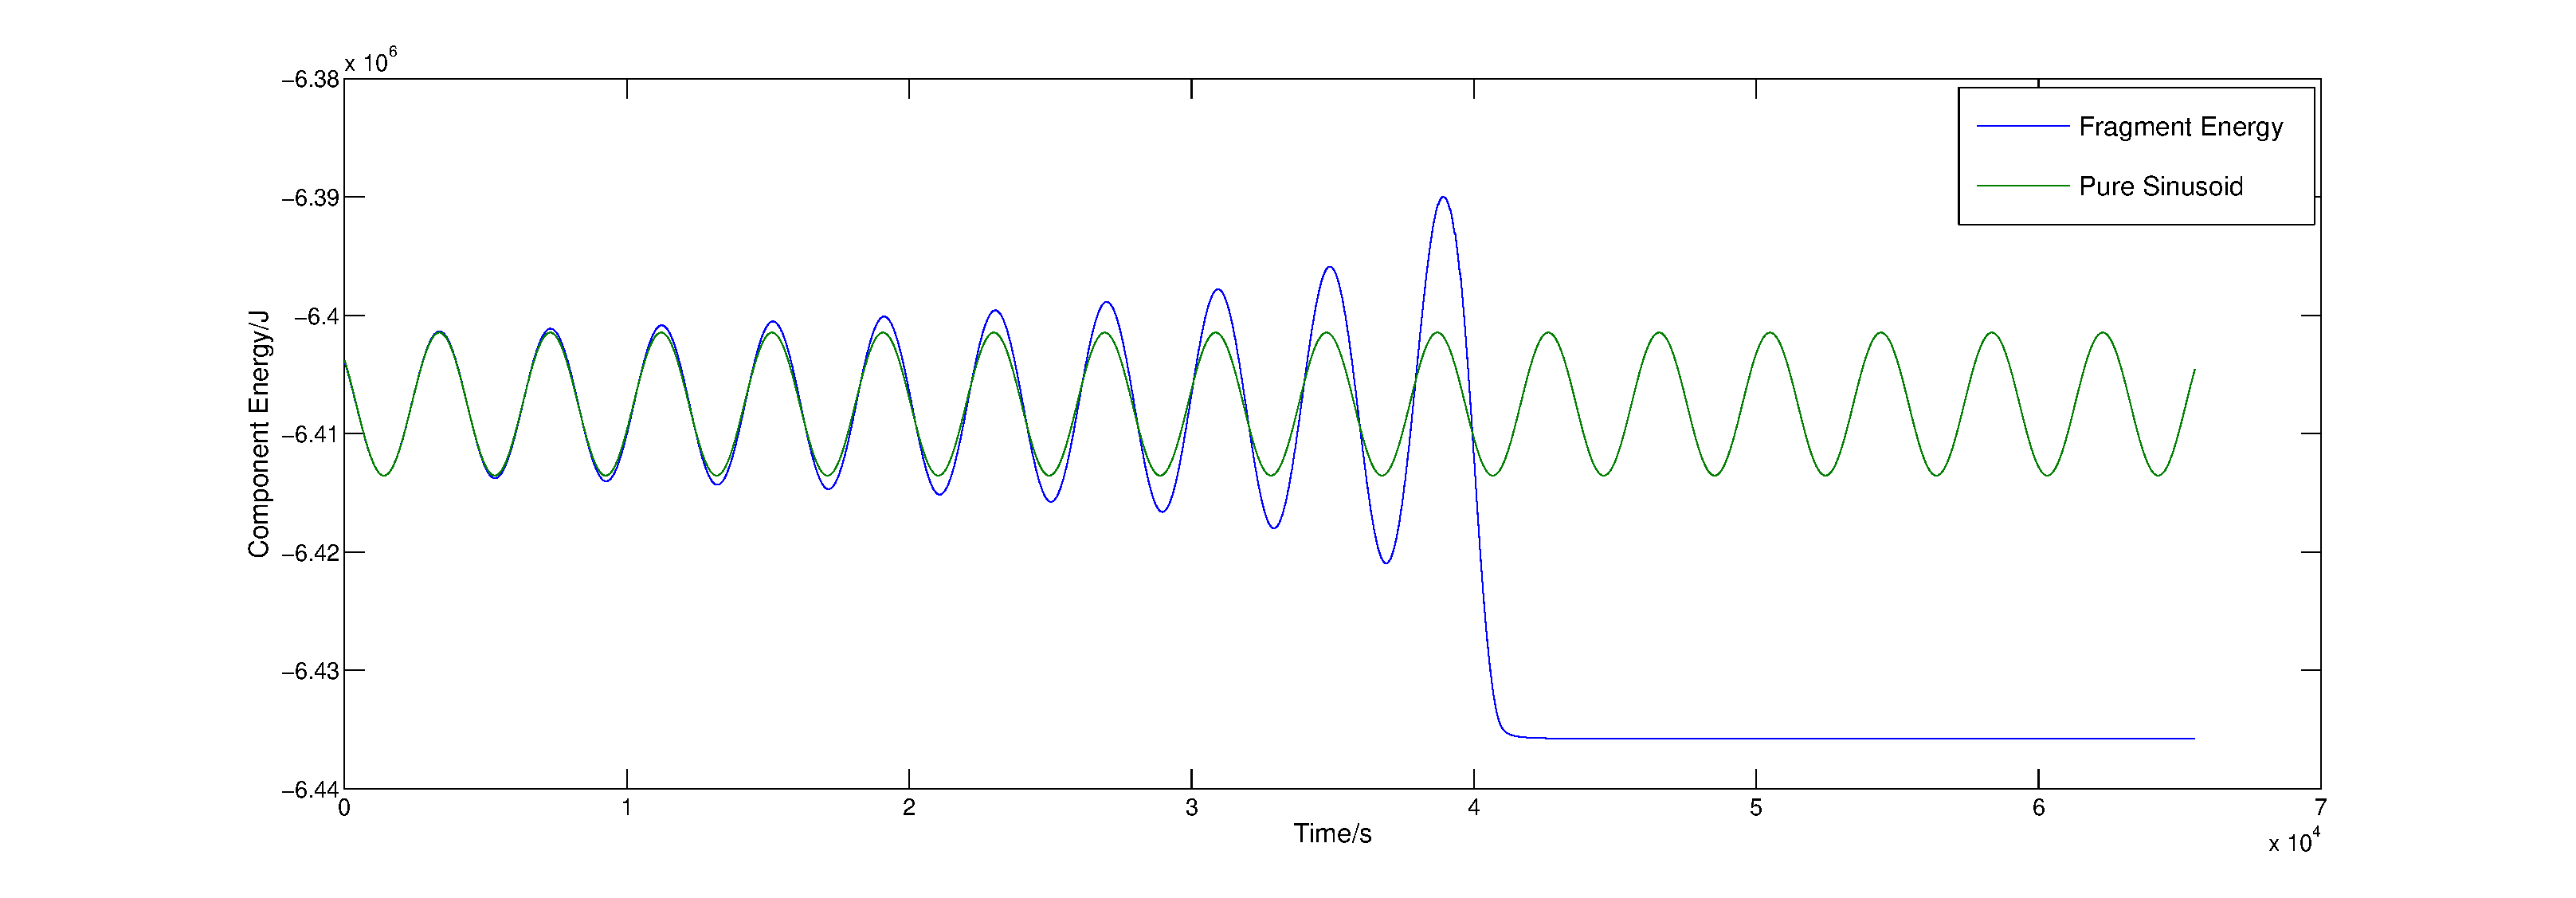
\includegraphics[width=\textwidth]{pure_sin.eps} 
\caption{Plot of the total energy of one components in a binary, plotted with a pure sine wave for comparison.} 
\label{fig:sin}
\end{figure}


Following this, numerical simulations of two boulders bound by a regolith bridge on a Parabolic trajectory were performed. 


\subsection{London Dispersion Forces}

For the small grain sizes considered in our regolith ($100\mu m$), the dominating force between particles is London Dispersion force. For point particles, the attractive and repulsive potentials are proportional to $1/r^6$ and $1/r^{12}$, respectively. However, for finite sized particles the formulation is more complicated. Hamaker \textbf{\emph{Reference}}. gives a derivation of the attractive potential between two spheres, calculated by the integral of the forces between infinitesimal point-particle elements over both spheres. In principle, this integral could be repeated for the repulsive term also. However, since we are using a soft-body collision method in our code including this term would provide no additional accuracy. Instead, we opt to use a Pseudo-potential method (Equation 9): for distances greater than a given cut-off radius $r_{cutoff}$, the full value of the Hamaker potential is used; for distances less than this a quadratic function is used instead. The quadratic used is set to have the same value and gradient as the Hamaker potential at the cut-off point, has a global minimum at some point $r_{min}$; similar to the soft-body collisions implemented this value is set to be less than the sum of the radii of the two spheres, thus allowing some overlap and "softening" the potential. 
\begin{equation}
V(r) = \left\{
\begin{array}{lr}
-\frac{A}{6}\left(\frac{2R_iR_j}{r^2-[R_i+R_j]^2}+\frac{2R_iR_j}{r^2-[R_i-R_j]^2}+\log\frac{r^2-[R_i+R_j]^2}{r^2-[R_i-R_j]^2}\right) & : r > r_{cutoff}\\
\frac{V'_{cutoff}}{2(r_{cutoff}-r_{min})}(r-r_{min})^2+V_{cutoff} - \frac{V'_{cutoff}(r_{cutoff}-r_{min})}{2} & : r \leq r_{cutoff}
\end{array}
\right.
\end{equation}
Ideally we wish to consider binary components with radii over 1 metre bound by a regolith bridge consisting of small ($100\mu m$) and medium ($1cm$) particles. However, the number of small particles which would have to be considered would make simulation of such a system not feasible. To overcome this, we first considered the binding effect between the small and medium particles. We established a simulation with two medium sized granules bound by a bridge of 510 small particles; the system was placed under rotation, initially with the rotation speed matching that of a purely gravitational circular orbit for the two medium granules. The rotation rate was gradually stepped up until the binding of the granules failed. The value of the Hamaker constant used in the simulations was then increased such that two medium sized granules had the same maximum rotation speed as when bound with the small particulate bridge. A factor of approximately 200 was found to be sufficient; this is roughly equal to the number of small particles in contact with each medium granule. Hence, the system considered for the regolith-bound simulations is comprised of the larger binary components bound by a bridge of 510 medium sized granules, with the additional effect of the small particles approximated by increased strength of the London Dispersion force.    
For the encounter simulations, a closest approach distance of 200 km is used, and the binary asteroid considered has a total diameter of 4 metres. Figure~\ref{fig:reg} shows the total energy results from the simulation, compared to those from a simulation of the same binary components and close approach distance but without the regolith bridge. The curves match closely before the fragmentation event; however when fragmentation occurs both binary components gain additional energy from the collapse of the binding regolith bridge. It can be seen that the amount of energy gained from the collapse is about $30\%$ of the difference in total energy between the two components.   
\begin{figure}[H]
\centering
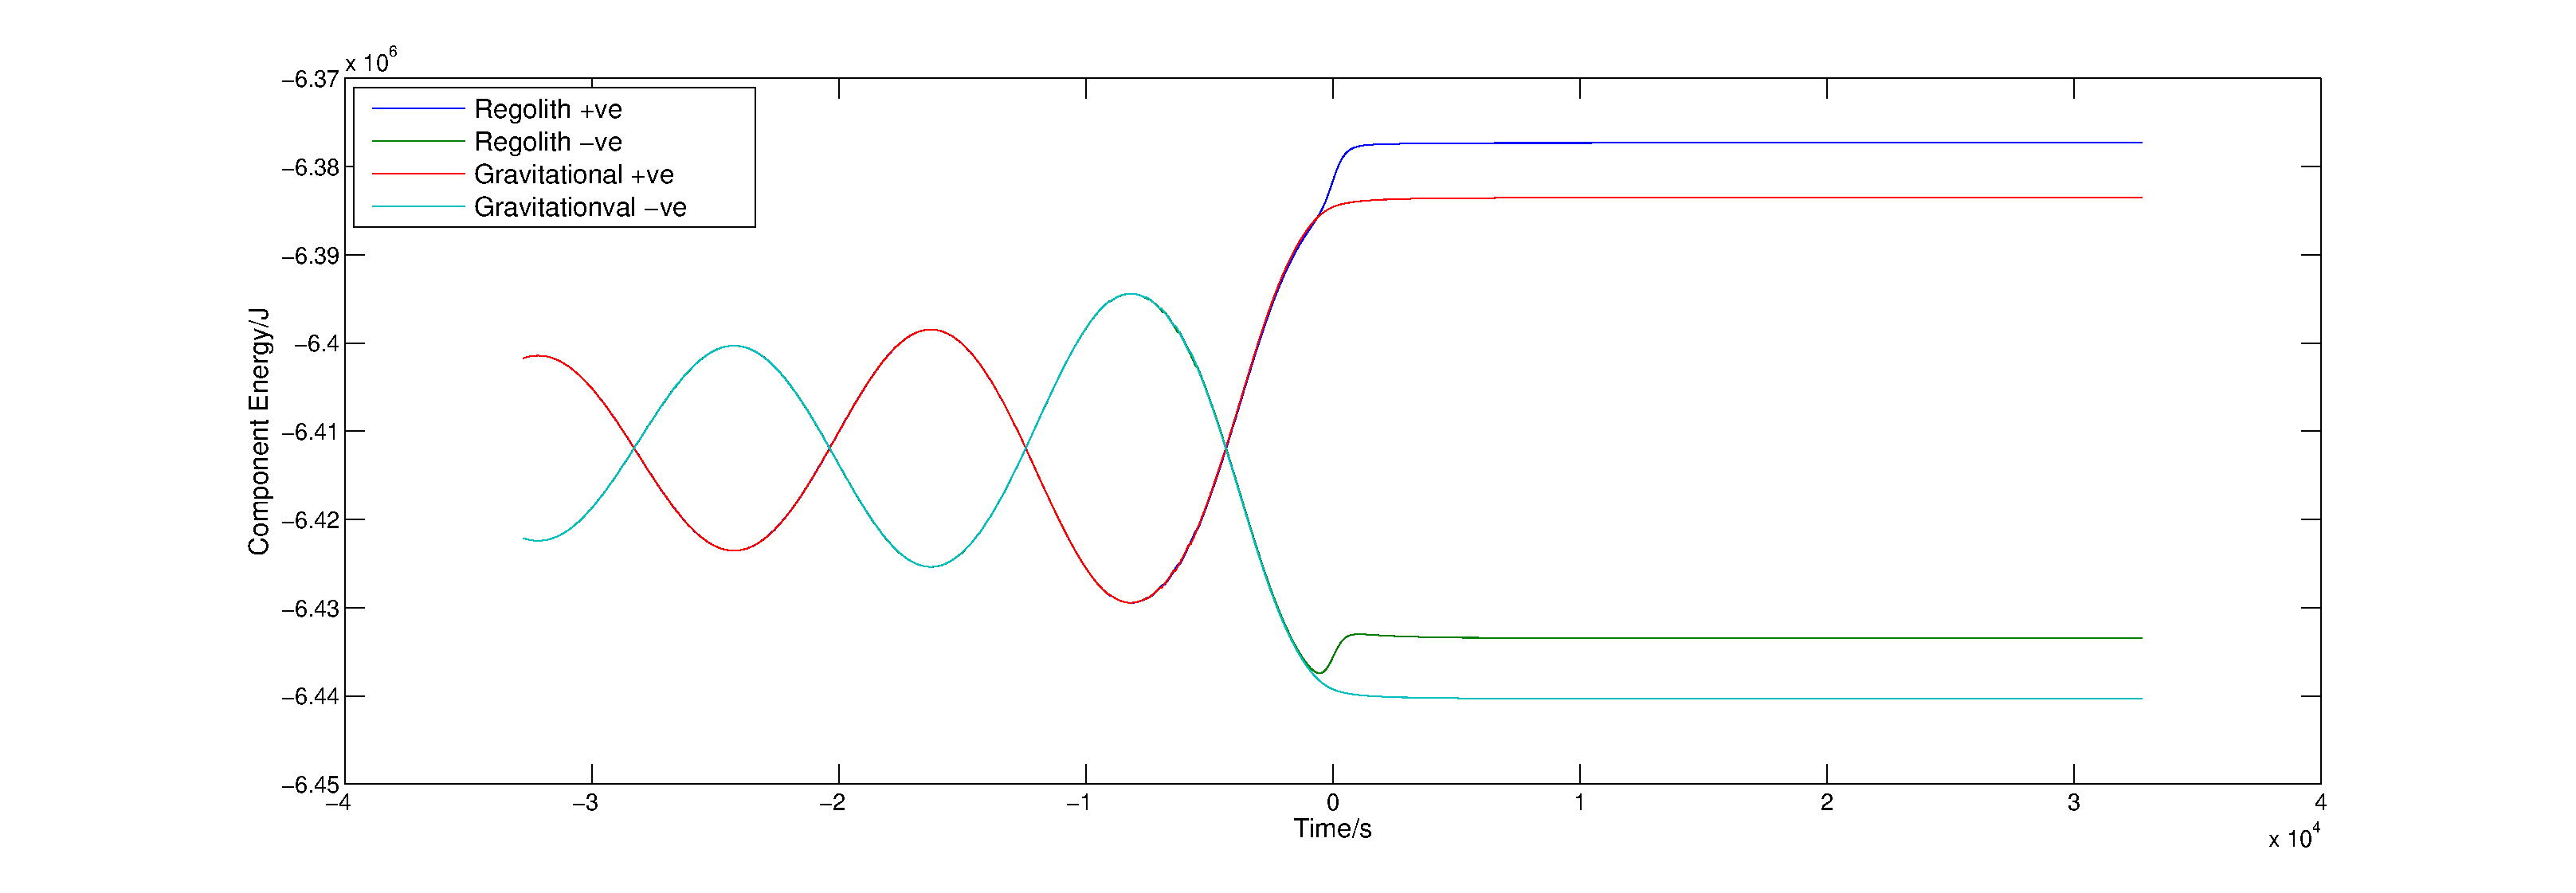
\includegraphics[width=\textwidth]{regolith_v_gravitational.eps} 
\caption{Plots of the Total energy of both components of the binary from numerical simulations; both for the purely graviational and the regolith-bound cases.} 
\label{fig:reg}
\end{figure}
\section{Conclusion}
We present a methodology to model contact binary asteroids bound by regolith during an encounter with a large body such as Earth. Any conclusions drawn from this research will allow for enhanced accuracy in the prediction of asteroid trajectories and allow for better planning in any mission to capture or deflect such an object.

\bibliographystyle{AAS_publication}   % Number the references.
\bibliography{references_me}   % Use references.bib to resolve the labels.

\section{Blah}
Similarly, considering only components orthogonal to $\vec{\rho}$ (and hence changes to the rotational speed of the pair) we obtain the following:
\begin{equation}
\ddot{\rho}_\bot = \dot{\omega}\rho +  {GM_\oplus}\left[\frac{\sin\theta}{R^{2}}-\frac{R\sin\theta}{R^{2}+2R\rho\cos\theta+\rho^{2}}\right]
\end{equation}



\end{document}
